\documentclass[journal abbreviation, manuscript]{copernicus}
\usepackage{comment} 

\begin{document}

 %% \ SECTION 3
\section{Use cases}

\begin{comment}
Andrew Comments:

Structure: just go through it, Use Case I, Use Case II, Use Case II. No Methods & Results section

go through it from front to back, explain what an NPZD model is.
"We recreate the NPZD model formulation by Anderson, in the model there is one .." describe equations in words. Then say See Anderson et al. or appendix X for full equations


%  quickly explain overview, explain methods for all of them shortly, with schematics, and put full system of equations & parameter tables in the Appendix!
\end{comment}

% PARAGRAPH STARTS HERE:
To showcase the utility of the phydra package for modelling marine ecosystems, we demonstrate three model implementations of varying complexity.
All model structures present highly idealised versions of marine ecosystems.\\

Use case 1 is a canonical NPZD ecosystem model embedded in a 'slab' physical setting. The specific implementation is adapted from the elegant EMPOWER model \citep{Anderson2015c}, with simplifications to the formulation of light-limited growth of phytoplankton.

Use case 2 presents a more complex size-structured food web embedded in a simple flow-through (chemostat) setting. It is a NPZ model that resolves many size-classes of phytoplankton and zooplankton and their trophic interaction. The model structure was inspired and adapted from \citet{Banas2011b}. 

Use case 3 embeds the complex food web of the second use case within the 'slab' physical setting of the first. Components and processes of each previous model instance are easily combined within the xarray-simlab framework, creating a completely different model, that shows oscillatory inter-annual fluctuations reminiscent of natural plankton populations. \\


The phydra package was designed specifically to create models of flexible dimensionality, as described in Section 2. For the presented use cases we focus on the dimension of ecosystem complexity in relatively simple zero-dimensional physical settings. Models can be run in one, two or three-dimensional physical schemes, by providing the appropriate setup grid and processes defining physical interactions between grid points. Our choice of zero-dimensional implementations was motivated by the fact that such physical schemes are much easier to set up and analyse. The online documentation of the phydra package provides simple examples of multi-dimensional marine ecosystem models.\\



% in final version, present: - jupyter notebook for each example, add links in text

\subsection{Forcing and verification data} \label{ForcingSection}

To simplify models of complex systems larger processes are not mechanistically implemented, but instead empirically represented as an external forcing. In two of the following use cases, we adapt a slab representation of ocean physics as defined by \citet{Evans1985ACycles}. The multi-dimensional ocean is reduced to two layers, where the upper layer provides a zero dimensional setting for our ecosystem model. The bottom layer is often assumed to contain a fixed concentration of nutrients (usually nitrate), but this can also vary with depth or time. There is constant exchange between the layers. Nutrients are usually mixing up into the upper layer, where they are consumed by phytoplankton. 

The fraction of all ecosystem components sinking to the bottom layer are lost from the system. These exchanges of water masses within this two-layered model ocean are driven by the empirically derived mixed layer depth (MLD). Additional common forcings that are used in slab models modify phytoplankton growth, e.g. metabolic rates and light harvesting via temperature and irradiance respectively. Such forcing can situate a slab model in a theoretical or any location in the global ocean. Compared to the natural habitat of marine plankton, the slab model is a radical simplification, however the resulting simulations can yield meaningful results that can be compared with bulk properties of the marine ecosystem. 

\subsubsection{Global nutrient, light and temperature climatologies as slab model forcing}
In line with the concept of phydra as a tool for rapid prototyping of marine ecosystem models, we provide with the package a set of global climatological model forcings. These forcings are derived from satellite data, World Ocean Atlas (WOA) 2018 data and a global MLD climatology kindly provided by Clément de Boyer Montégut.

WOA data provides objectively analyzed climatological mean depth profiles of nutrients (nitrate, phosphate \& silicate) and temperature on a one-degree longitude/latitude grid \cite{Garcia2019WORLDSilicate}. The values have been interpolated from data collected in the World Ocean Database and provide an empirical estimate of the biogeochemical conditions in areas of the global ocean throughout the year.\\

The MLD climatology is an updated version of the original climatology presented in  \citet{deBoyerMontegut2004MixedClimatology}, collecting data up until 2014 and with a modified criterion for MLD. Spatial resolution of the climotology is on a 2 \unit{°} longitude/latitude grid. The analysis of profile data combines a fixed threshold criterion for temperature (0.2 \unit{°C}) and a variable threshold criterion in density (equivalent to a 0.2 \unit{°C} decrease). MLD is diagnosed as the minimum calculated depth of both criterion for each station. This ensures that both temperature and salinity are homogeneous within the mixed layer, and compensated or barrier layers do not skew the values of MLD. This combined MLD criterion corresponds to a proxy of overturning extent depth over a few days, which lends this MLD value very well as the forcing that drives the upwelling of deeper nutrients into the upper mixed layer in slab physics (Clément de Boyer Montégut, personal communication).\\

In addition to the oceanographic and biogeochemical parameters, the provided set of global forcings includes a global climatology of irradiance from satellite data. The NASA satellite MODIS-aqua provides the most up-to-date global climatologies of photosynthetically active radiation (PAR) \cite{MODIS-Aqua2018NASAGroup}. The data product estimates incident PAR at the ocean surface using ..., which can be used to calculate light-availability to phytoplankton within the modelled upper layer.\\

By combining satellite PAR, MLD climatology and WOA data, we can experimentally run a slab model built in phydra in (almost) any location of the ocean. MLD can be used as an empirical forcing for mixing in our slab models. Average nutrient concentration below the mixed layer, extracted from the WOA 2018 climatologies, can be used to provide a more realistic estimate of nutrient supply at certain locations throughout the year. This was done using ... and taking into account 50 \unit{m} below closest available climatological MLD value. The final 1 \unit{°} gridded data product can be accessed via Github [provide link] and is easily integrated with models build using the phydra package. 

From this global forcing dataset, we chose two representative locations in the Atlantic ocean (see Figure \ref{phydraforcing}). These two locations were chosen for their contrasting environment. Temperate with deep MLD in winter, light and temperature variable. Tropical relatively stable conditions throughout the year, lower nutrient supply through mixing. \\


\subsubsection{Satellite chlorophyll and nutrient climatologies as verification data}
Model verification is a very difficult process
- it usually takes specific tailoring of the model to the data, or vice versa \cite{Schartau2017}
- a good fit, does not mean a correct model \cite{RykielJr1996}\\

BUT, still is a basic test of model function, and for demonstration purposes.
We chose to use the Nutrient data from the WOA climatologies for nutrient concentration in the upper layer.

Additionally, we use chlorophyll climatologies from MODIS-aqua (cite!) and 

carbon-based phytoplankton size classes calculated from ocean color estimates of the particle size distribution \cite{Kostadinov2016Carbon-basedDistribution}.\\

The provided dataset provides an easy way to compare model output to empirical data. 

The data are highly aggregated climatologies, of poor temporal resolution (monthly). We follow this path to provide a universally useful, simple tool for marine ecosystem model development. For more specific model implementation and hypothesis testing it would be highly recommended to use local data.\\


\subsection{Use case 1: NPZD slab model}

The specific NPZD slab model implementation for our Use Case 1 was adapted from \citet{Anderson2015c}. For a schematic of the model structure, see figure \ref{phydraschematics_1} (a).

The model contains the name-defining four ecosystem components: Nutrient, phytoplankton, zooplankton and detritus. The only resolved nutrient in this system is nitrate. The biomass of all other state variables is measured in the common model currency \unit{µM} of Nitrogen. Four forcings affect the model dynamics: nitrate below the mixed layer ($N_0$), depth of the mixed layer ($MLD$), photosynthetically active incident radiation ($PAR$), average temperature above the mixed layer depth ($T_{MLD}$). The forcings are interpolated monthly climatologies as described in section \ref{ForcingSection}. See figure \ref{phydraforcing} for the two locations and specific forcings applied here.
For the full set of equations, please see the Appendix.\\

% Nutrient dynamics
$N_0$ determines the possible nutrient supply to the ecosystem. Mixing of nutrients is a function of a constant mixing parameter, $N_0$, $N$ and the value and derivative of $MLD$, following \citet{Evans1985ACycles}. In contrast to other components, mixing affecting the nutrient is a positive term adding to $N$ along the gradient between $N_0$and $N$. The general direction of transport is from a nutrient-rich bottom layer to the upper layer supporting phytoplankton growth.

In slab models, the concentration of nutrient in the bottom layer $N_0$ is often assumed to be fixed. In reality there is quite often a gradient of concentration over depth, and this can be represented using functions of nutrient over depth \citep{Frost1987GrazingSpp.}. In this study we use an empirical climatology as the forcing $N_0$, that is the result of combining WOA 2018 data with MLD climatology (see section \ref{forcingdatasect}). The specific variable used is Nitrate+Nitrite. This data provides the contrasting seasonal dynamics for the temperate and tropical location (see figure \ref{phydraforcing}).

The derivative of $MLD$ affects mixing only when the mixed layer depth is increasing, as 
The change in depth of the mixed layer, described by the derivative of $MLD$, provides an estimate of mixing intensity. When $MLD$ is shallowing (negative), the loss of component concentration is balanced with the increasing concentration due to a decreasing model volume. A deepening $MLD$ dilutes all components and drives the mixing of nutrient into the upper layer. 

% Phytoplankton dynamics
The only condition where mixing can bring the nutrient concentration $N$ to approach $N_0$ is when phytoplankton growth is severely limited. In the model, growth of $P$ is modified by three factors: Temperature, nutrient uptake and light harvesting. Multiplied by the maximum intrinsic growth rate $\mu_P$ and the current $P$ biomass, the growth flux is computed. Temperature dependence of phytoplankton growth is calculated as the Eppley constant \citep{Eppley1972TemperatureSea}, with an exponential equivalent to a $Q_{10}$ of 1.895.
In slab model simulations with a seasonally deep mixed layer, the most limiting factor during these events is often the light-dependence of phytoplankton growth. The light-limiting term is calculated via Steele's formulation \ref{Steele1962EnvironmentalSea}. Incident irradiance is supplied by the $PAR$ climatological forcing. Integrated light availability in the upper layer is calculated via Beer's law, dependent on $MLD$ and the sum of extinction coefficients of water and $P$ biomass. Phytoplankton light limitation is further defined by a n$I_{opt}$ parameter, that describes where the available light saturates photosynthesis, which equals phytoplankton growth in this simplified model.
When sufficient light is available, phytoplankton will consume nutrients. All nutrients consumed are directly incorporated into biomass. This uptake/growth rate is defined by a Monod (or Michaelis-Menten) function, showing a saturating behaviour at high nutrient availability. The maximum rate is defined by a parameter, $k_N$ the half-saturation constant for $N$ uptake. 
% here phytoplankton mortalities

% Zooplankton dynamics
In this simple model zooplankton $Z$ is not affected by environmental factors, such as light or temperature. We assume that zooplankton can actively maintain in the upper mixed layer and only compute diluting effects of $MLD$ deepening, but no other mixing terms.  
So unaffected, the only task awarded to zooplankton is to graze phytoplankton (well, and to die). 
% here zooplankton grazing!
% here zooplankton mortalities


% Detritus dynamics
% here how grazing and mortality add to detriuts
% and remineralisation
In addition to mixing loss, detritus is affected by a sinking flux. 



A complete description of model mechanisms and presentation of equations is given in Appendix 1.\\


differences from EMPOWER: \\
Very simple model,
irradiance from satellite, not trigonometric equations. we treat light in much less detail, so say that for a more detailed treatment of light in a slab model, see \cite{Anderson2015c}

Our modifications to phytoplankton grwoth formulation, zooplankton mixing, as well as the treatment of forcing were adapted from the PhytoSFDM model \cite{Acevedo-Trejos2016}.
% can I say that Esteban? it is true

EMPOWER was inspired by \cite{Fasham1990a}, we stand in a long line of models. 

We hope that this simple NPZD slab model can be used as a teaching model in a similar vein to EMPOWER. The modular structure of phydra processes allows for accessible experimentation with parameterisation and model setup. 


% In EMPOWER i noticed a problem with the shape model output presented in the paper and too large model time steps (due to for loop code structure, not odeint adaptive solving).. is that something I should mention, or simply forget?

\subsusection{Model Structure: NPZD}
explain model structure in words, reference equations in appendix

\subsubsection{Physical setting: slab}
explain slab physics, equations in appendix



\subsubsection{NPZD slab model results}
show and explain results, as simple as possible, full parameters/sensitivity analysis in appendix?


\subsection{Use Case 2: Size-structured chemostat model}

This specific system could be described as a chemostat, where constant nutrient addition drives the growth of multiple state variables of phytoplankton and zooplankton. Each plankton state variable is assigned a size measured as the equivalent spherical diameter (ESD). The ESD determines the nutrient uptake parameters, growth rates and grazing susceptibility via size-based allometries taken from meta-analysis of laboratory data.

\subsection{Model Structure: size-structured NPZ}

\subsubsection{Physical setting: chemostat}


\subsubsection{Model results}


\subsection{Use Case 2: Size-structured chemostat model}

\subsection{Model Structure: size-structured NPZD}



\subsubsection{Physical setting: slab}

\subsubsection{Model results}


\clearpage
% Figures

%%f
\begin{figure*}[t]
\includegraphics[width=15cm]{Figures/firstdraft_plots/01_forcing_labeled.pdf}
\caption{(a) Map shows locations of the two comparative model runs. Each square is of side length 4° centered on 47°N ,-20°E and 0°N,-20°E respectively. Environmental forcings are averaged across area. (b) Forcing is shown: Mixed Layer Depth (MLD), Nitrate below the Mixed Layer (N_0), Photosynthetically Active Radiation (PAR) and temperature averaged across the Mixed Layer (T_{MLD})}
\label{phydraforcing}
\end{figure*}



%%f
\begin{figure*}[t]
\includegraphics[width=15cm]{Figures/firstdraft_schematics/02__schematics_NPZDandChemostat.pdf}
\caption{(a) Model schematic of NPZD slab model for example 1. Model structure and parametrisation is adapted
from \citet{Anderson2015c} (b) Model schematic of size-structured NP_{40}Z_{40} trophic model for use case 2.
Model structure and parameterisation is adapted from \citet{Banas2011b}.}
\label{phydraschematics_1}
\end{figure*}


%%f
\begin{figure}[t]
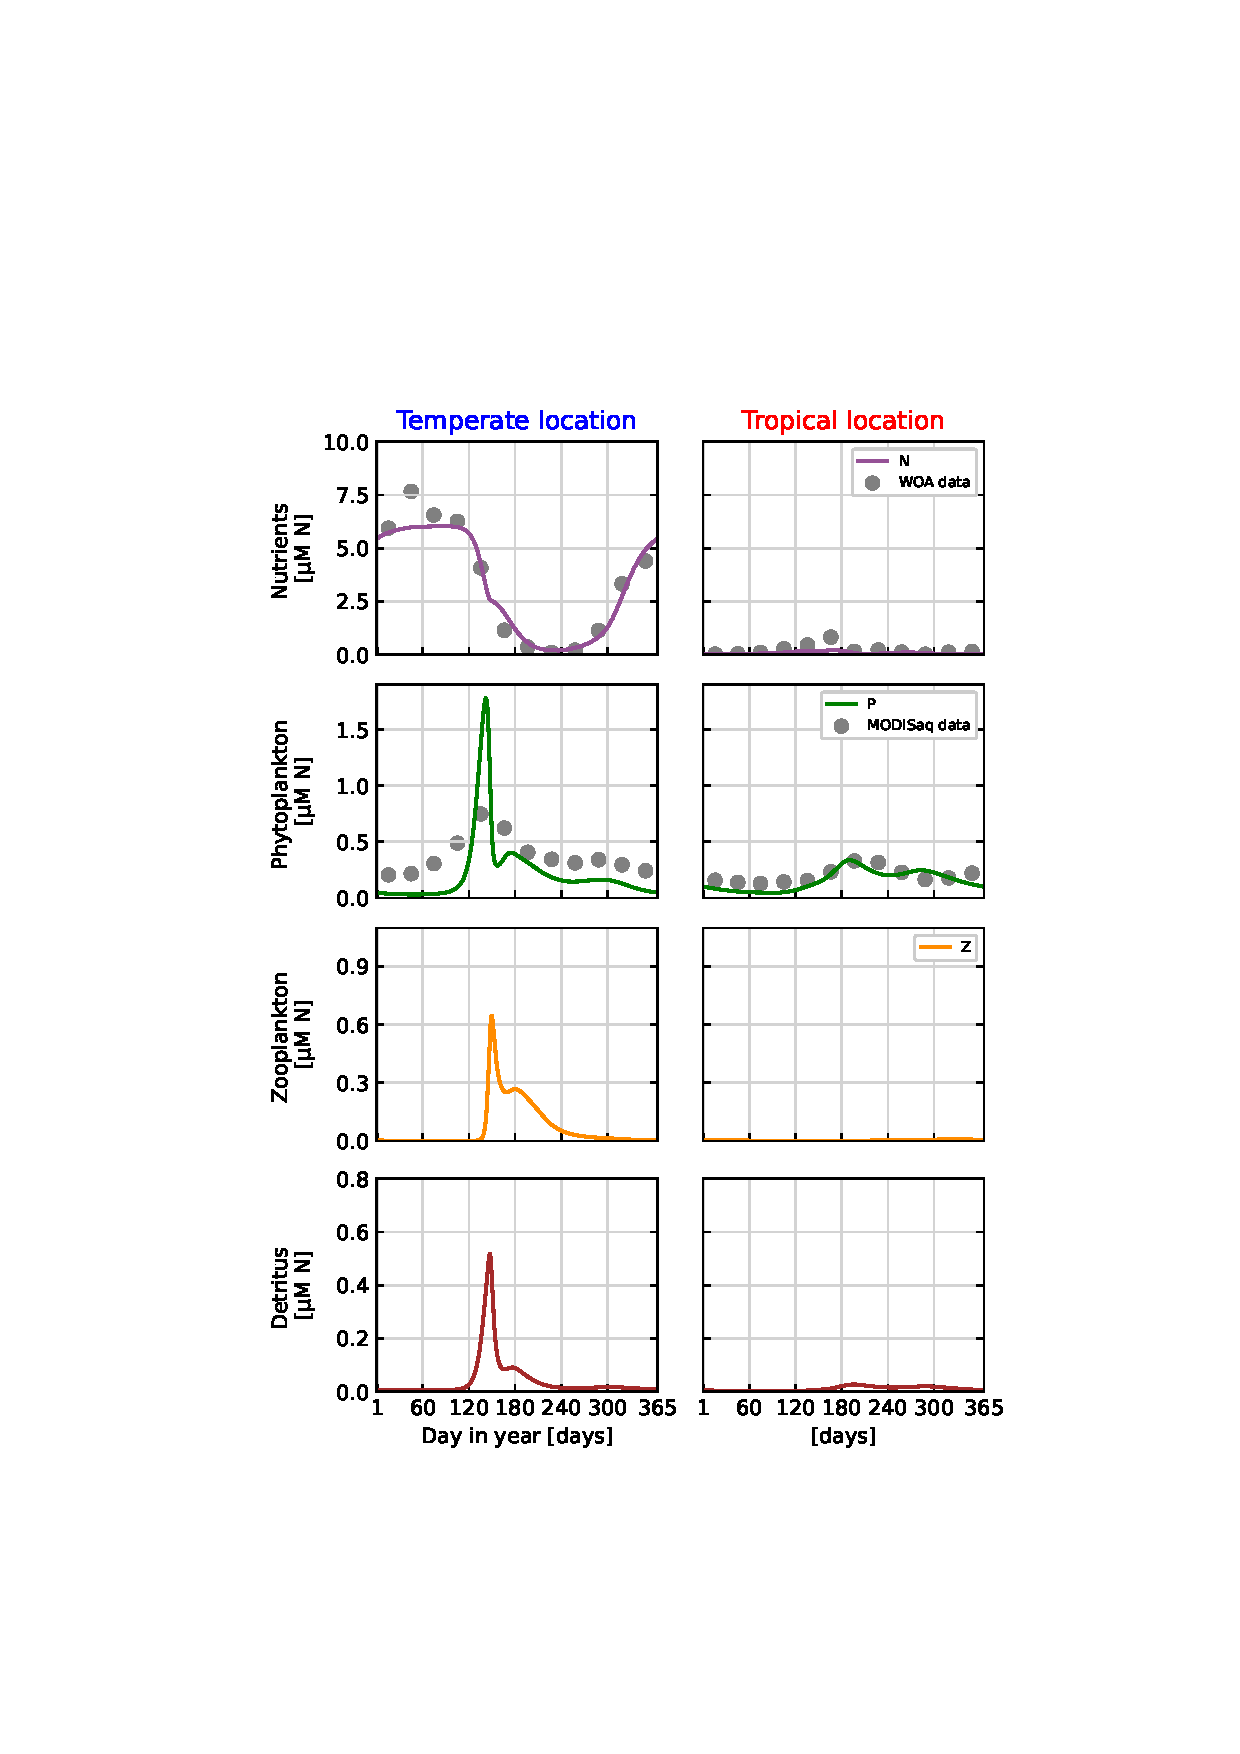
\includegraphics[width=6cm]{Figures/firstdraft_plots/02_NPZDslab.pdf}
\caption{Model output for the two locations of the NPZD slab model is shown between the two sites.}
\end{figure}

%%f
\begin{figure}[t]
\includegraphics[width=6cm]{Figures/firstdraft_plots/03_chemostat.pdf}
\caption{Model output for the size-structure chemostat model. Plot is a recreation (same model setup & parameters) of a plot in \citet{Banas2011b}}
\label{ASTroCAT_plot}
\end{figure}

%%f
\begin{figure*}[t]
\includegraphics[width=10cm]{Figures/firstdraft_schematics/03__schematics_SizeStructSlab.pdf}
\caption{Model schematic of size-structured NP20Z20 slab model for use case 3.}
\label{phydraschematics_3}
\end{figure*}



%%f
\begin{figure*}[t]
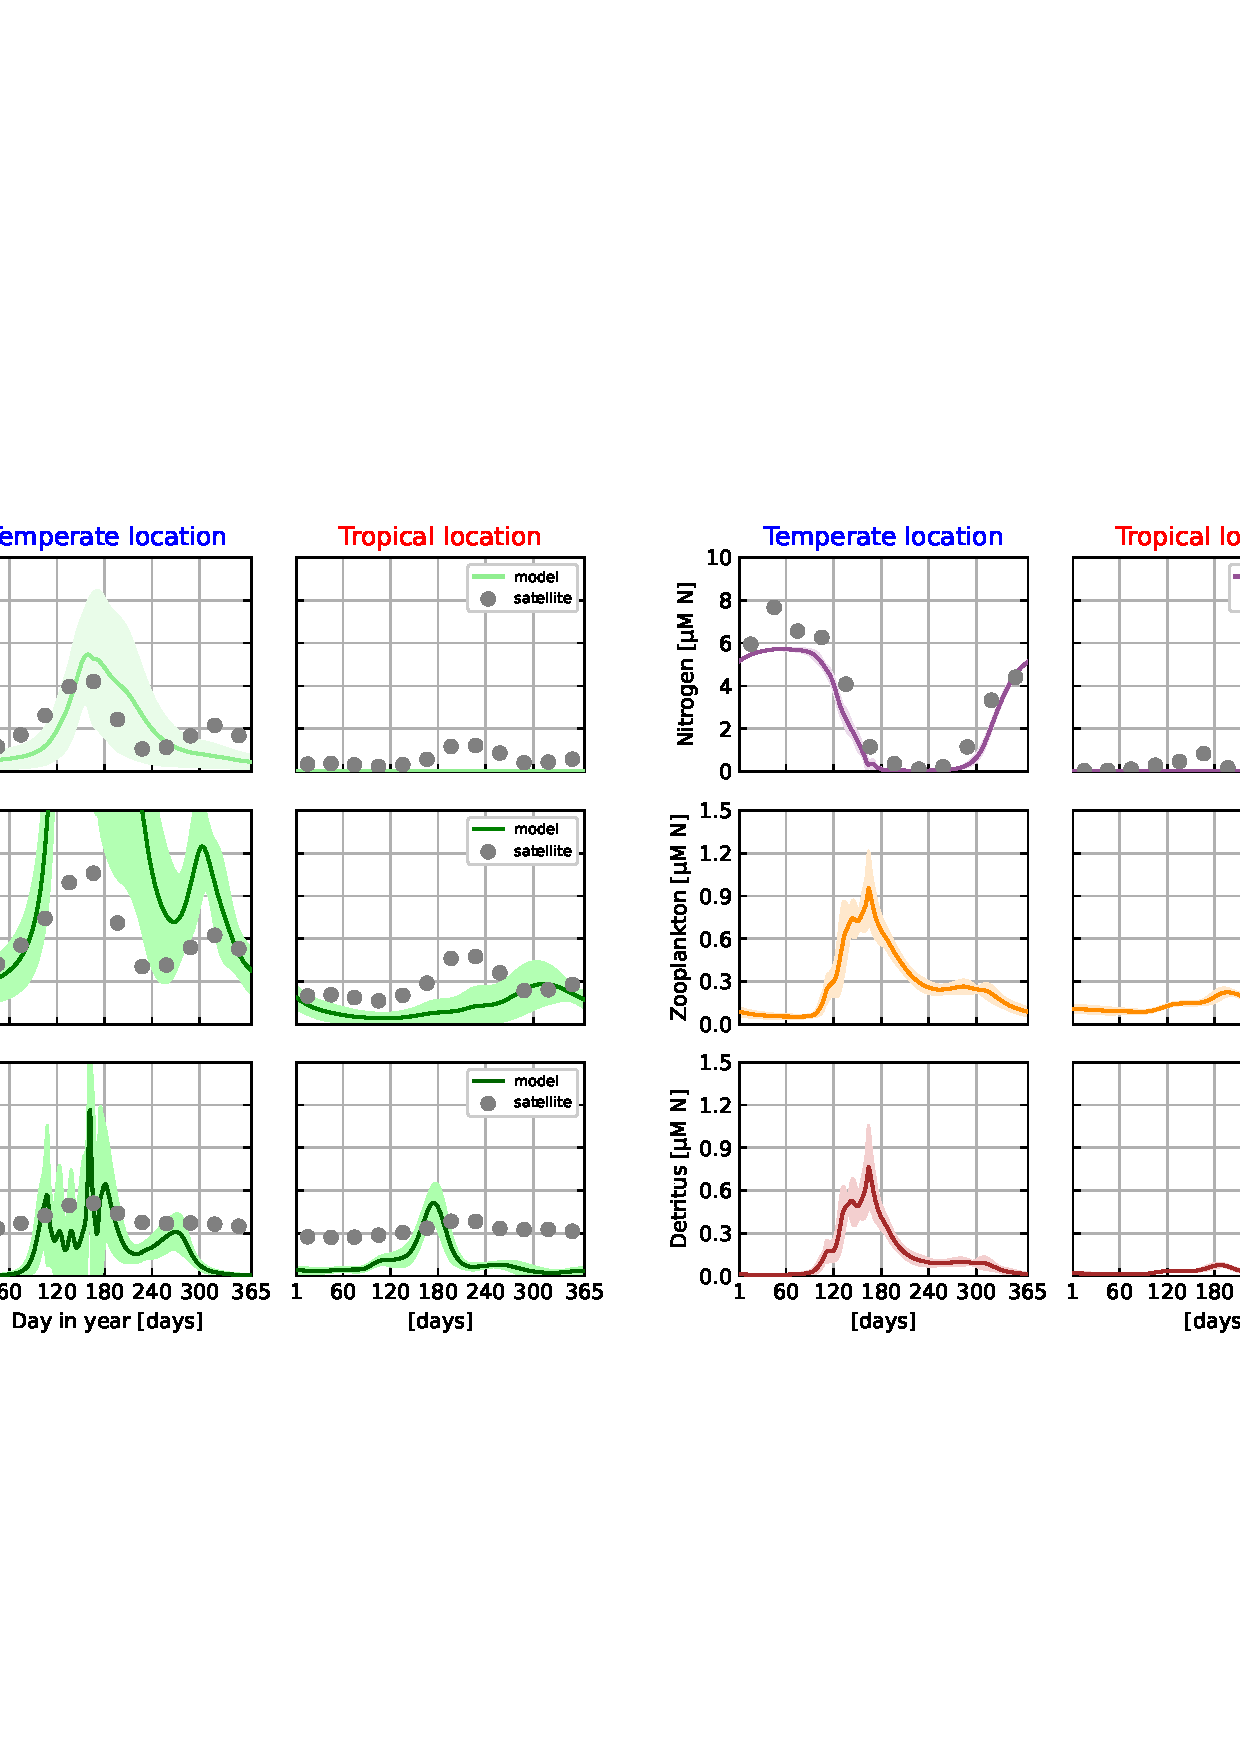
\includegraphics[width=12cm]{Figures/firstdraft_plots/04_sizestruct_slab.pdf}
\caption{Model output for the two locations of the size-structured NP_{20}Z_{20}D slab model}
\label{ASTroCAT_plot}
\end{figure*}
% Tables


% needs to be added to render sections
\bibliographystyle{copernicus}
\bibliography{references.bib}

\end{document}